\chapter{Improving convergence between MM and QM by application of a bias} \label{Chapter:biasing_potentials}

\section{Introduction}

By using hybrid Monte Carlo \cite{hybrid_mc} a desired potential can be sampled by using a cheaper reference file.  In the current case, QM/MM is the desired potential and MM is the cheap reference potential.  The acceptance criterion for such a method is,

\begin{equation} \label{eq:acceptance}
\ A_{ij}= \exp [ - \beta (( U_{QM}^f + U_{KIN}^f ) - (U_{QM}^i + U_{KIN}^i))] \\.
\end{equation}

$U_{QM}^i$ is the QM/MM potential energy of snapshot $i$, the current snapshot.  $U_{KIN}$ is the kinetic energy, for snapshot $i$ this is taken from a Gaussian distribution, for $f$ this is extracted from the underlying MD simulation.  The MD is used as an engine to generate uncorrelated structures quickly and is run with constant Hamiltonian energy (i.e. the microcanonical ensemble).  By using a small MD time step of 0.25 fs the errors in the integrator will be negligible and the difference in the QM/MM Hamiltonian used within equation \ref{eq:acceptance} can be rewritten as,


\begin{eqnarray}
\ \Delta H &=& (E_{QM}^f+E_{KIN}^f) - (E_{QM}^i+E_{KIN}^i) \\
\ &=& E_{QM}^f - E_{QM}^i + E_{KIN}^f - E_{KIN}^i \\
\ &=& E_{QM}^f - E_{QM}^i + E_{MM}^i - E_{MM}^f \\
\ &=& (E_{QM}^f - E_{MM}^f) - (E_{QM}^i - E_{MM}^i) .
\end{eqnarray}

This shows that the acceptance of structures into the QM/MM ensemble is related to the level of overlap between the MM and QM/MM.  Two potential energy surfaces were generated for methanol by freezing all degrees of freedom except the C-O bond and the C-O-H angle to illustrate the effect that this inexact overlap of phase space can have on the energy difference.

\begin{figure}
\begin{center}
 \scalebox{0.8}{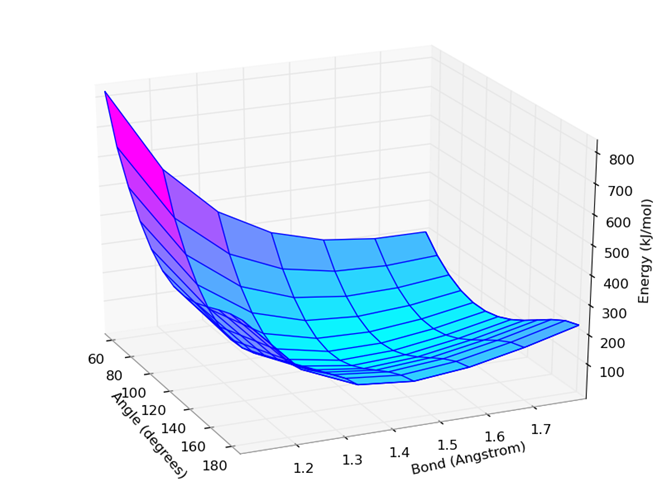
\includegraphics{QM_PES_methanol.png}}
 \caption{QM potential energy surface for methanol}\label{fig:QM_PES_methanol}
 \end{center}
\end{figure}

\begin{figure}
\begin{center}
 \scalebox{0.8}{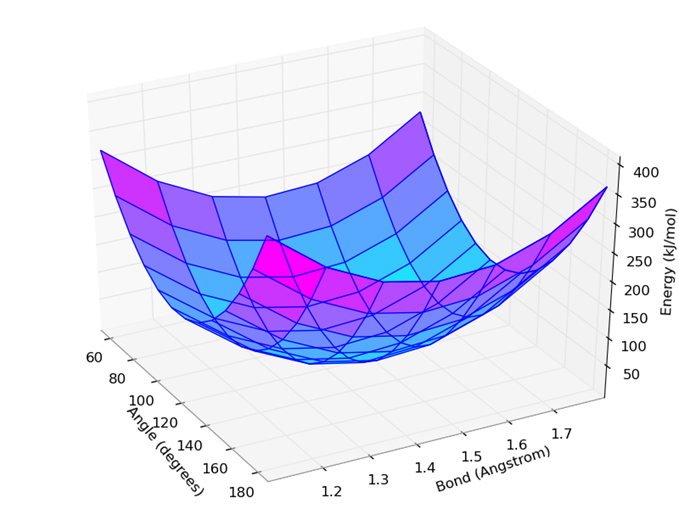
\includegraphics{MM_PES_methanol.png}}
 \caption{MM potential energy surface for methanol}\label{fig:MM_PES_methanol}
 \end{center}
\end{figure}

\begin{figure}
\begin{center}
 \scalebox{0.8}{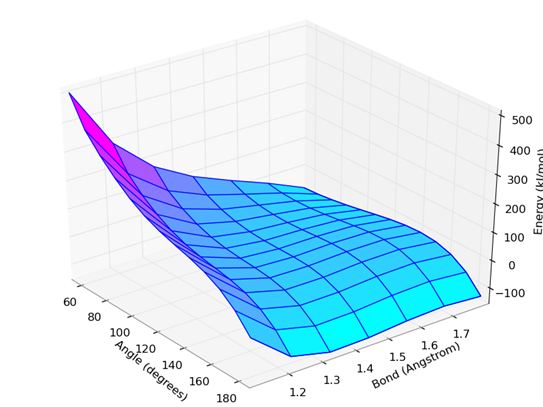
\includegraphics{QM-MM_PES_methanol.png}}
 \caption{QM - MM energy difference surface for methanol}\label{fig:QM-MM_PES_methanol}
 \end{center}
\end{figure}

From figure \ref{fig:QM_PES_methanol} and \ref{fig:MM_PES_methanol} it is clear to see the poor overlap which results in figure \ref{fig:QM-MM_PES_methanol}.  The regions of negative energy difference have been caused by the different types of surface (Morse like vs Harmonic).  Once a hybrid Monte Carlo simulation is performed, an unfair weight is given to these low energy difference structures, regardless of the position on the QM potential energy surface, so for the above example, this is a high energy QM structure that is being used to describe the ensemble and this will bias the ensemble average.  

Notice however, that the position of the minimum is the same for both the MM and QM surfaces.  A bias can be applied to ensure better sampling of the minimum and can ensure that the simulation will not get stuck in a low energy difference region.  The use of biasing potentials within free energy calculations is not novel \cite{umbrella_sampling, MM_to_QM_bias, TI_LE_free_energy, non-boltz_ti}.  Reference \cite{MM_to_QM_bias} uses the energy difference to bias the free energy, then unbiases by using the relationship described in reference \cite{umbrella_sampling},

\begin{equation} \label{eq:unbias}
\ \langle X \rangle = \frac{\langle X \exp (\beta \omega) \rangle_{bias}}{\langle \exp(\beta \omega) \rangle_{bias}} \\.
\end{equation}
%
Where $X$ is the property of interest, $\omega$ is the applied bias.

By including the bias into the acceptance criterion a biased ensemble can be generated.  The acceptance criterion is then,

\begin{equation}
\ A_{ij} = \exp[ - \beta \{[( U_{QM}^f + \omega^f ) - U_{MM}^f ] - [(U_{QM}^i+ \omega^i) - U_{MM}^i]\}] \\.
\end{equation}

By setting $\omega$ to a simple function, such as $\frac{1}{2} \kappa (\Delta U- \langle \Delta U \rangle)^2$ there are only two unknowns to identify: $\kappa$ and $\langle \Delta U \rangle$.  $\Delta U$ in this case is the difference in the QM and MM energies i.e. $\Delta U = U_{QM} - U_{MM}$.  Identifying the average energy difference is a process that is updated at every proposed snapshot.  The process to find the constant $\kappa$ is slightly more complicated.

After X steps of the simulation being stuck in a low energy difference, a bias is applied such that if the next snapshot proposed was equal to the average energy difference, it would be accepted. i.e., 

\begin{equation}
\ \langle \Delta U \rangle =  (\Delta U^i)+ \omega^i \\.
\end{equation}

Then using the value of $\omega^i$ the value for $\kappa$ is found,

\begin{equation}
\ \kappa=\frac{2 \omega^i}{(\Delta U^i - \langle \Delta U \rangle)^2}
\end{equation}

The value for $\omega^f$ is then calculated using $\kappa$. $\kappa$ will remain unchanged unless the simulation gets stuck in a low energy difference snapshot for X steps again.

After 100 steps of hybrid Monte Carlo, the average energy difference and the constant $\kappa$ are fixed.

In practice, once the biased ensemble has been generated, the property of interest to unbias in equation \ref{eq:unbias} is the energy difference required for TI,

\begin{eqnarray}
\ \left\langle \frac{\partial U}{\partial \lambda} \right\rangle &=& \frac{\left\langle \frac{\partial U}{\partial \lambda} \exp[-\beta \omega] \right\rangle_{bias}}{\left\langle \exp[-\beta \omega] \right\rangle_{bias}} \\
\ U &=& \lambda U_{QM} + (1-\lambda) U_{MM} \\
\ \frac{\partial U}{\partial \lambda} &=& U_{QM} - U_{MM} .
\end{eqnarray}

For the perturbation between the QM/MM and QM the Zwanzig equation is used, the property to unbias in the case is the following,

\begin{equation}
\ \left\langle  \exp[ -\beta ( U_{QM}-U_{QM/MM}) \right\rangle = \frac{\left\langle  \exp[ -\beta ( U_{QM}-U_{QM/MM})] \exp[\beta\omega] \right\rangle_{bias}}{\left\langle \exp[\beta\omega] \right\rangle_{bias}} \\.
\end{equation}

%\section{Methods}

%N2 equilibration

%acceptance to QM ensemble

\section{Results}

In order to validate the proposed method, N$_2$ in vacuum was selected to act as a test system.  By using such a simple test case, the unbiased simulation can be performed and the results can be compared.  Because the unbiased simulation can be performed, it is unlikely that the simulation will get stuck in a low energy difference well, therefore a bias will never be applied.  In order to circumvent this, a manual bias value of 0.5 was applied.  The initial comparison between the obtained average energy difference for the unbiased and biased simulation can be seen in table \ref{table:N2_comparison_1}.

\begin{center}
\begin{table*}[ht]
{
\hfill{}
\begin{tabular}{c | c | c }
\hline 
 & Unbiased & Biased \\ 
\hline 
 Average energy difference (kJ/mol) & -52430.70 & -52434.95 \\
\hline 
\end{tabular}}
\hfill{}
\caption{Comparison of average energy difference between the QM and MM at $\lambda=1$}
\label{table:N2_comparison_1}
\end{table*}
\end{center}

The initial results shown in the above table display a 4 kJ/mol difference between the average energy difference obtained from the biased and unbiased simulations.  This result was surprising considering only a single degree of freedom is present within N$_2$.  To discover the reason for this difference the equation used to unbias the biased simulation was examined,

\begin{equation} \label{eq:unbias_equation}
\ \left\langle \frac{\partial U}{\partial \lambda} \right\rangle = \frac{\left\langle \frac{\partial U}{\partial \lambda} \exp[ \beta \omega] \right\rangle_{bias}}{\left\langle \exp[ \beta \omega] \right\rangle_{bias}} \\.
\end{equation}

There are two aspects to this equation, the numerator and the denominator.  By considering the average for these values as the number of included snapshots is increased, an idea of how converged the results are can be obtained. 

\begin{center}
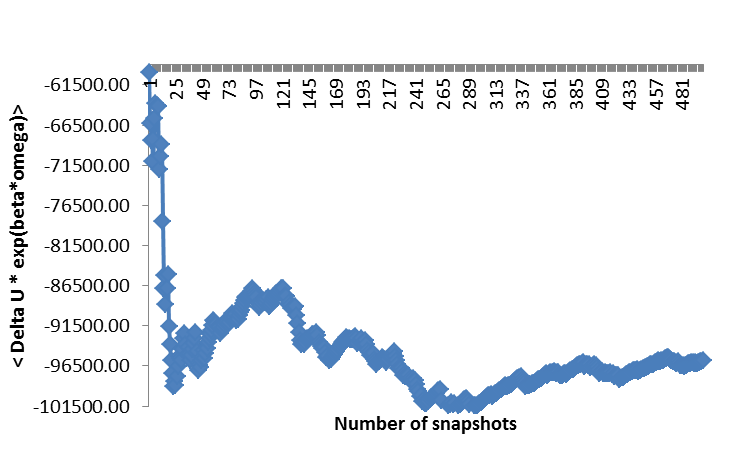
\includegraphics[width=15cm]{N2_numerator.png}
%\captionof{figure}{Calculating the numerator of equation \ref{eq:unbias_equation} as the number of snapshots is increased}\label{fig:N2_numerator}
\end{center}

\begin{center}
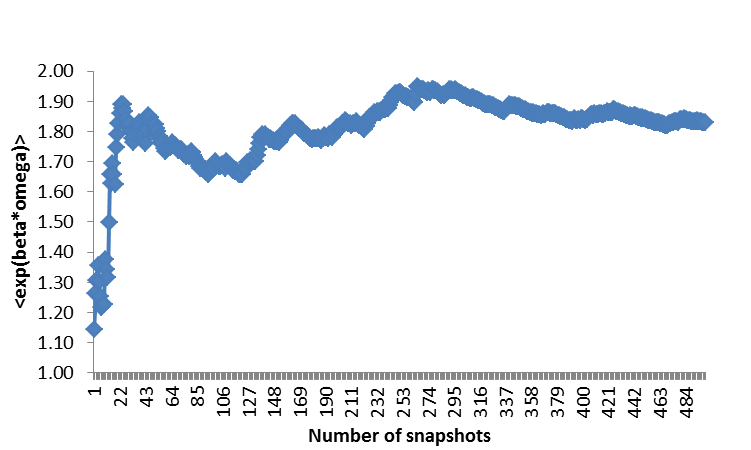
\includegraphics[width=15cm]{N2_denominator.png}
%\captionof{figure}{Calculating the denominator of equation \ref{eq:unbias_equation} as the number of snapshots is increased}\label{fig:N2_denominator}
\end{center}

The denominator very quickly converges to between 1.8 and 1.9, however, the numerator continues to show large fluctuations throughout the simulation.  The cause of the fluctuations within the numerator can be attributed to the large energy differences between the QM and MM energies.

Additional tests were then run, these include running an additional 500 hybrid Monte Carlo steps using the same constant (0.5) and center of bias as the previous simulation, using a smaller constant (0.1) and finally, doubling the equilibration steps within hybrid Monte Carlo to 200.


\begin{center}
\begin{table*}[ht]
{
\hfill{}
\begin{tabular}{c | c | c | c }
\hline 
  & 0.5 constant (cont) & 0.1 constant & 200 step equilibration \\ 
\hline 
 Average energy difference (kJ/mol) & -52434.82 & -52434.96 & -52434.92 \\
\hline 
\end{tabular}}
\hfill{}
\caption{Comparison of average energy difference between the QM and MM at $\lambda=1$ varying the constant and equilibration length}
\label{table:N2_comparison_2}
\end{table*}
\end{center}

The results for the additional test simulations in table \ref{table:N2_comparison_2} do not match the average energy difference obtained from the unbiased simulation in table \ref{table:N2_comparison_1}.  Interestingly, all the results that were obtained from a biased simulation compare very well to one another, falling within a range of 0.1 kJ/mol.  This excellent convergence led to the re-examination of the terms in equation \ref{eq:unbias_equation}, following the same process as before, but using the average of the unbiased energy difference.

\begin{center}
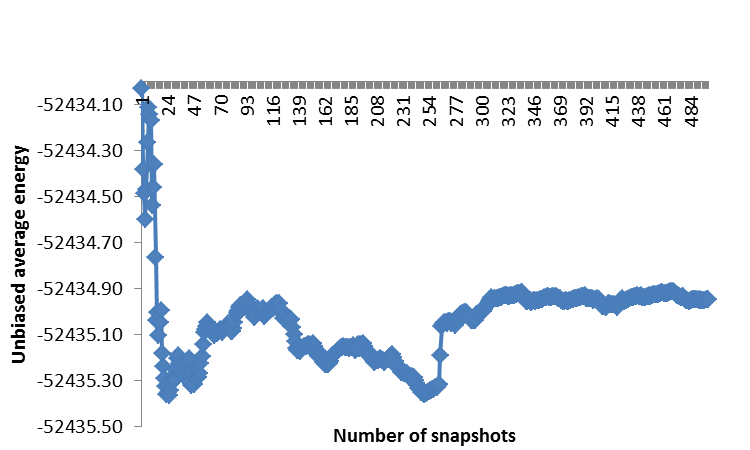
\includegraphics[width=15cm]{N2_unbasied_energy.png}
%\captionof{figure}{Calculating the unbasied energy as the number of snapshots is increased
\label{fig:N2_unbiased_energy}
\end{center}

Figure \ref{fig:N2_unbiased_energy} shows a fast convergence of the energy difference, showing a fluctuation of less than 0.2 kJ/mol within 300 snapshots.

A more complex test system, ethanol in vacuum, was then used.  Again this system can be used within the unbiased simulation so a manually set bias of 0.5 was applied and the standard 500 hybrid Monte Carlo steps were used.

\begin{center}
\begin{table*}[ht]
{
\hfill{}
\begin{tabular}{c | c | c}
\hline 
  & Unbiased simulation & Biased simulation \\ 
\hline 
 Average energy difference (kJ/mol) & -81546.81
 & -81544.51 \\
\hline 
\end{tabular}}
\hfill{}
\caption{Comparison of average energy difference between the QM and MM at $\lambda=1$ for ethanol in vacuum}
\label{table:Ethanol_comparison_1}
\end{table*}
\end{center}

The results in table \ref{table:Ethanol_comparison_1} again show a small difference between the average energy difference obtained from the biased and unbiased simulations.  In order to check convergence, the biased simulation was continued for an additional 1000 hybrid Monte Carlo steps.


\begin{center}
\begin{table*}[ht]
{
\hfill{}
\begin{tabular}{c | c }
\hline 
   & Biased simulation (cont) \\ 
\hline 
 Average energy difference (kJ/mol) & -81544.22 \\
\hline 
\end{tabular}}
\hfill{}
\caption{Comparison of average energy difference between the QM and MM at $\lambda=1$ for ethanol in vacuum}
\label{table:Ethanol_comparison_2}
\end{table*}
\end{center}

Performing an additional 1000 steps shows no change in the average energy difference.  As before, the average energy difference was calculated as a function of the number of snapshots included and the result is shown in figure \ref{fig:Ethanol_unbiased_energy}.  


\begin{center}
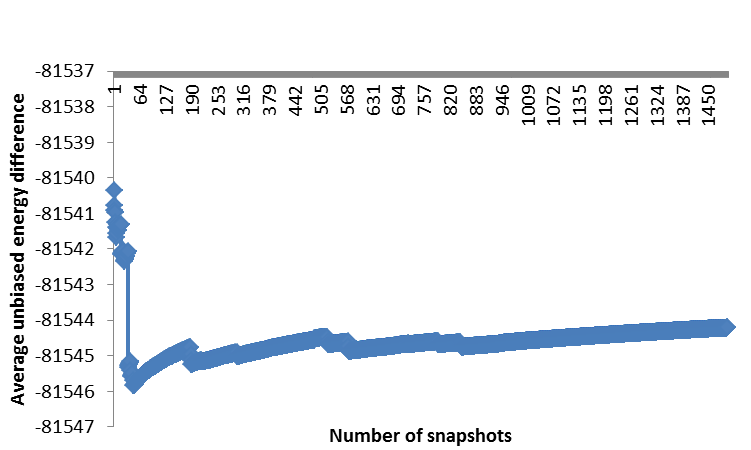
\includegraphics[width=15cm]{Ethanol_unbasied_energy.png}
%\captionof{figure}{Calculating the unbasied energy as the number of snapshots is increased}
\label{fig:Ethanol_unbiased_energy}
\end{center}

The slight ``jumps'' present within the above figure show the first signs of ``sawtooth'' behaviour, characteristic of poor sampling\cite{good_practice_free_energy}.  To identify whether these jumps can be overcome with sampling, alanine dipeptide was used.  As a structure that cannot be sampled using the unbiased method, only biased simulations were performed, three repeats were run in order to check for convergence.  The results can be seen in table \ref{table:Alanine_dipeptide_energy}.


\begin{center}
\begin{table*}[ht]
{
\hfill{}
\begin{tabular}{c | c | c | c }
\hline 
   & Run 1 & Run 2 & Run 3 \\ 
\hline 
 Average energy difference (kJ/mol) & -245749.95 & -245755.24 & -245759.52 \\
\hline 
 Center of bias (kJ/mol) & -245743.87 & -245740.52 & -245741.59 \\
\hline 
 Constant & 0.34299 & 0.13284 & 0.07103 \\
\hline
 Acceptance \% & 30.6 & 40.8 & 36.2 \\
\hline
\end{tabular}}
\hfill{}
\caption{Comparison of simulation details for three repeats of alanine dipeptide in vacuum}
\label{table:Alanine_dipeptide_energy}
\end{table*}
\end{center}


It is clear to see from table \ref{table:Alanine_dipeptide_energy} that convergence has not been achieved, with a range of around 10 kJ/mol between values.  However, the center of the bias for each simulation, had a much lower range with values.  A simulation was then performed with a high constant of 10.  As expected the acceptance rate dropped to 7.4\%.  The final result was -245743.68, which is within 6 kJ/mol of run 1.  This may be attributed to the higher constant within run 1, indeed, it from table \ref{table:Alanine_dipeptide_energy} it is apparent that the higher constant, the closer to the unbiased average energy will be to the bias center.  Convergence for the high constant simulation for alanine dipeptide can be seen in figure \ref{fig:alanine_dipeptide_high_constant}.  To test if the unbiased average energy can be reproduced if the same bias center and constant is used, run 1 was performed again.  This time an unbiased average energy of -245751.31 was achieved.


\begin{center}
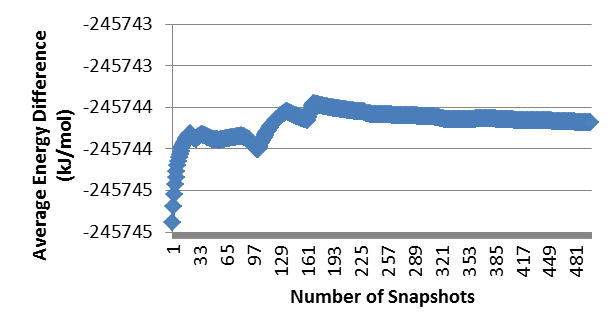
\includegraphics[width=15cm]{alanine_dipeptide_unbasied_energy_high_constant.png}
%\captionof{figure}{Calculating the unbasied energy as the number of snapshots is increased for alanine dipeptide in vacuum with a constant of 10}
\label{fig:alanine_dipeptide_high_constant}
\end{center}

Each simulation run involves quantum simulations that take between 10-15 minutes of cpu time on 4 cores.  In order to find whether using a bias will work for different systems without the time consuming simulations a numerical test was designed.  Random values were taken from a Gaussian distribution using the Marsaglia polar method\cite{Maraglia_polar_method} using a constant of 0.3, a bias center of -80,000 and varying the standard deviation.  The computational cost of this numerical test is negligible, so 1,000,000 values were collected for each run.  The results are shown below.


\begin{center}
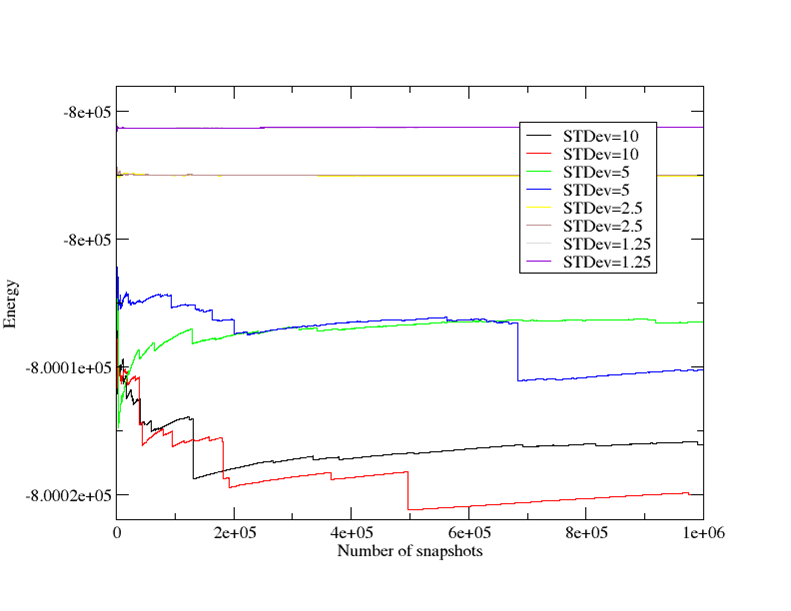
\includegraphics[width=15cm]{numerical_test.png}
%\captionof{figure}{Results for the numerical test, bias center at -80000 with a constant of 0.3}
\label{fig:numerical_test}
\end{center}


Figure \ref{fig:numerical_test} shows that for a standard deviation 5 or above convergence is never achieved.  Energy ranges increases as more degrees of freedom are included, this leads to the conclusion the biased method will not converge for systems of biological interest.


\section{conclusions}

By including a bias into hybrid Monte Carlo previous systems that could not be sampled can be, with a relatively high acceptance rate.  However, unless the system has few degrees of freedom the final unbiased energy will not converge.  

In order to improve this a guiding potential that better represents the quantum ensemble should be used.
